% =====================================================================
% IEEE JBHI regular paper -- STRUCTURAL SCAFFOLD ONLY
%
% This file contains NO scientific prose. Every section is a placeholder
% carrying (a) what belongs there, (b) the authoritative artifact the
% content must come from, and (c) the claim constraints that apply.
%
% paper/main.tex is untouched historical scaffolding with stale framing.
% Draft from this file and from docs/JBHI_DRAFTING_MANIFEST.md, not from
% main.tex.
%
% -------------------------------------------------------------------
% !! TEMPLATE ACQUISITION REQUIRED -- AUTHOR ACTION !!
%
% This repository does NOT contain an IEEEtran class file, and no TeX
% toolchain is installed on the machine this scaffold was written on, so
% the document has not been compiled. No formatting rule has been invented
% here.
%
% Before drafting:
%   1. obtain the current IEEEtran template from the IEEE Author Center
%      (IEEEtran.cls, and the IEEE journal bibliography style);
%   2. place IEEEtran.cls alongside this file or install it;
%   3. confirm the class options below against the template IEEE ships --
%      the \documentclass line is the conventional one for IEEE journals
%      but MUST be checked against the current JBHI instructions;
%   4. confirm the required bibliography style name.
% -------------------------------------------------------------------
% =====================================================================

\documentclass[journal]{IEEEtran}

\usepackage{graphicx}
\usepackage{amsmath}
\usepackage{amssymb}
\usepackage{booktabs}
\usepackage{url}
\usepackage[hidelinks]{hyperref}

\graphicspath{{../outputs/figures/jbhi_final/}}

\begin{document}

% =====================================================================
% FRONT MATTER -- every field below is a placeholder. Do not guess any.
% =====================================================================

\title{[TITLE --- must not claim priority; see
       docs/FINAL\_CLAIM\_EVIDENCE\_MAP.md. The subject is the
       protocol-by-initialisation interaction, not a model comparison]}

\author{[AUTHOR LIST]%
  \thanks{[AUTHOR ORDER]}%
  \thanks{[AFFILIATIONS]}%
  \thanks{[CORRESPONDING AUTHOR: name, email, postal address]}%
  \thanks{[ORCID]}%
  \thanks{[FUNDING]}%
}

\maketitle

% ---------------------------------------------------------------------
\begin{abstract}
% ~0.25 page. Structure: problem, gap, design, primary result with
% numbers, and the explicit non-claim.
%
% MUST state the primary interaction with its Holm-adjusted p-values on
% both domains, and MUST state that no difference was demonstrated under
% full fine-tuning without calling that equivalence.
%
% Source: outputs/tables/JBHI_PRIMARY_INTERACTION.csv
% Allowed/forbidden wording: docs/FINAL_CLAIM_EVIDENCE_MAP.md
[ABSTRACT]
\end{abstract}

\begin{IEEEkeywords}
[INDEX TERMS --- e.g. foundation models, transfer learning, domain
 generalisation, diabetic retinopathy, model evaluation. Check the IEEE
 taxonomy before finalising.]
\end{IEEEkeywords}

% =====================================================================
\section{Introduction}
% ~0.8--1.0 page.
%
% Frame: frozen linear probing is the cheap standard for ranking
% foundation-model representations; whether that ranking predicts
% fine-tuned behaviour is an untested assumption.
%
% The contribution is the DIRECT WITHIN-LINEAGE PROTOCOL-INTERACTION
% evaluation. It is NOT "the first comparison of RETFound with
% SSL-ImageNet" -- that comparison is in the original RETFound paper.
%
% Use "to our knowledge", never "first".
% Source: docs/LITERATURE_NOVELTY_AUDIT.md sections 0 and 4.
[INTRODUCTION]

% =====================================================================
\section{Related Work}
% ~0.6--0.8 page total. Source: docs/LITERATURE_NOVELTY_AUDIT.md section 2.

\subsection{Retinal Foundation Models}
% RETFound and its lineage; RETFound-Green; pre-training data effects.
% Must state that RETFound's own paper already compares against an
% SSL-ImageNet baseline with matched fine-tuning.
% Cite: zhou2023retfound, engelmann2025retfoundgreen,
%       zhou2026pretrainingdata
[RELATED WORK A]

\subsection{Foundation-Model Evaluation Protocols}
% Frozen probing vs fine-tuning; where protocol and model identity are
% confounded in prior work.
% Cite: poyrazer2026frozen, engelmann2025retfoundgreen,
%       zhou2026pretrainingdata, gulrajani2021domainbed
[RELATED WORK B]

\subsection{Cross-Dataset DR Generalization}
% External evaluation and label efficiency.
% Cite: yew2026labelefficiency, poyrazer2026frozen, li2019ddr,
%       porwal2018idrid
[RELATED WORK C]

% =====================================================================
\section{Materials and Methods}
% Methods + Experimental Design together: ~1.7--2.0 pages.

\subsection{Datasets and Provenance}
% Four DR datasets; LODO design; splits; the integrity controls.
% MUST include: EyePACS is in RETFound's published pretraining corpus and
% is a SOURCE domain here; this is disclosed and is NOT target leakage.
% MUST include: the EyePACS folder physically contains all 3,662 APTOS
% images and the loader rejects them by filename.
% Source: docs/JBHI_DATASET_PROVENANCE.md
% Table: TABLE I
[METHODS A]

\subsection{Matched Pretraining Lineage}
% ViT-L/16; RETFound continues MAE pretraining from the ImageNet-MAE
% checkpoint on retinal CFP. Same architecture, same lineage.
% Checkpoint identities and hashes: docs/JBHI_EVIDENCE_FREEZE.md section 5
% Cite: zhou2023retfound, he2022mae, dosovitskiy2021vit, deng2009imagenet
% Figure: Fig. 1
[METHODS B]

\subsection{Downstream Adaptation Protocols}
% Frozen linear probe; partial FT (last 4 of 24 blocks); full FT
% (303,306,757 trainable parameters, asserted at runtime). One fixed
% recipe, no per-domain tuning.
[METHODS C]

\subsection{Evaluation Metrics}
% QWK primary. Secondary: macro F1, balanced accuracy, severe-error rate,
% MAE grade, within-1-grade, macro AUROC, ECE, NLL.
% Cite: cohen1968kappa, brier1950verification, guo2017calibration,
%       naeini2015ece, geifman2017selective, cao2020coralordinal
[METHODS D]

\subsection{Statistical Analysis}
% Crossed seed x case bootstrap = UNCERTAINTY INTERVAL, not a test.
% Paired seed-level t-test = FORMAL TEST.
% Holm = multiplicity adjustment, across the two interaction tests only.
% Exact sign-flip = distribution-free sensitivity, floor 0.0625 at n=5.
% Seed SD and sign count = descriptive stability diagnostics.
%
% Do NOT use the phrase "two-bar rule".
% Qualifying effects are "statistically supported under the study's
% inferential framework".
% Where interval and test disagree, the formal test governs.
% Source: docs/JBHI_EVIDENCE_FREEZE.md section 7
[METHODS E]

% =====================================================================
\section{Experimental Design}

\subsection{Frozen Linear Probing}
% 10 seeds (42,1,2,3,4,5,6,7,8,9), three held-out domains.
[DESIGN A]

\subsection{Partial Fine-Tuning}
% Last 4 of 24 blocks, 5 seeds (42,1,2,3,4), three held-out domains.
[DESIGN B]

\subsection{Full Fine-Tuning}
% All encoder parameters + head, 5 seeds, DDR and APTOS only.
% IDRiD full FT was NOT run and is not imputed anywhere.
[DESIGN C]

\subsection{External-Domain Protocol}
% Target labels never used for selection, early stopping, hyperparameter
% choice or temperature scaling. Temperature fitted on source validation.
[DESIGN D]

\subsection{Confirmatory APTOS Replication}
% CHRONOLOGY GUARDRAIL -- state it exactly this way:
%   1. the DDR full-FT experiment was specified, frozen, run and OBSERVED;
%   2. APTOS was THEN specified as a confirmatory replication, with the
%      recipe copied unchanged and the analysis written before any APTOS
%      target outcome was inspected;
%   3. Holm adjustment across the two domains is applied for final
%      two-domain reporting.
%
% Do NOT imply the two-domain family was pre-specified before DDR was seen.
% Source: docs/JBHI_EVIDENCE_FREEZE.md section 10
[DESIGN E]

% =====================================================================
\section{Results}
% ~1.7--2.0 pages. Every number from an authoritative table; see
% docs/JBHI_DRAFTING_MANIFEST.md.

\subsection{Frozen Evaluation}
% Ten-seed descriptive estimates. MUST note the direction is NOT uniform:
% DDR and APTOS favour ImageNet-MAE, IDRiD favours RETFound.
% Source: JBHI_MASTER_RESULTS.csv, seed_set = all-10
[RESULTS A]

\subsection{Adaptation-Depth Effects}
% Frozen -> partial -> full, common-five seeds only.
% Language: ATTENUATION, not reversal. On APTOS the mean ordering never
% changes sign; a mean reversal may be described for DDR descriptively and
% must not be generalised.
% Source: JBHI_MASTER_RESULTS.csv, seed_set = common-5
% Figure: Fig. 2 -- Table: TABLE II
[RESULTS B]

\subsection{Primary Protocol Interaction}
% THE PRIMARY RESULT. Both domains, Holm-adjusted, never pooled.
% Source: JBHI_PRIMARY_INTERACTION.csv
% Figure: Fig. 3 -- Table: TABLE III
[RESULTS C]

\subsection{Full-Fine-Tuning Comparison}
% Both domains: no difference demonstrated. NOT equivalence.
% DDR needs explicit handling: its crossed interval excludes zero while
% the seed-level test does not reject (p = 0.1035); the formal test
% governs and nothing is claimed.
% Source: JBHI_MASTER_RESULTS.csv, protocol = full
% Figure: Fig. 5
[RESULTS D]

\subsection{Secondary Reliability Analyses}
% Secondary metrics are exploratory and uncorrected. The two APTOS metrics
% below 0.05 (macro AUROC, ECE) are NOT claimed.
% Source: aptos_secondary_outcomes.csv,
%         full_finetune_secondary_outcomes.csv
% Supplementary figures: S4, S5, S6
[RESULTS E]

% =====================================================================
\section{Discussion}
% ~0.8--1.0 page (with Limitations, 1.0--1.2 total).
% What a frozen probe does and does not tell you; relation to
% poyrazer2026frozen (frozen arm) and yew2026labelefficiency (full-FT arm).
% Forbidden claims are listed in docs/FINAL_CLAIM_EVIDENCE_MAP.md.
[DISCUSSION]

% =====================================================================
\section{Limitations}
% MUST include, at minimum:
%   L1 -- IDRiD contributes no full-FT evidence; the interaction is a
%         two-domain result and nothing is imputed for IDRiD.
%   L2 -- the two-domain family is a post-hoc pairing (see chronology).
%   L3 -- EyePACS exposure, disclosed, not target leakage.
%   plus: one architecture, one adaptation budget, five seeds, sign-flip
%         floor 0.0625, runs not bit-reproducible by design.
% Source: docs/FINAL_CLAIM_EVIDENCE_MAP.md
[LIMITATIONS]

% =====================================================================
\section{Conclusion}
% ~0.25 page. No new claim may appear here that is not already supported
% in Results.
[CONCLUSION]

% =====================================================================
% BACK MATTER -- placeholders, do not guess
% =====================================================================

\section*{Data Availability}
[DATA AVAILABILITY LANGUAGE --- four public datasets; per-dataset access
 conditions; confirm redistribution is not implied. See
 docs/DATASET\_CITATION\_NOTES.md]

\section*{Code Availability}
[CODE REPOSITORY / DOI --- whether this repository is released, licence,
 and a commit-pinned archive DOI]

\section*{Ethics Statement}
[ETHICS DETERMINATION --- wording must come from the institution. The
 study uses only previously published, de-identified public datasets]

\section*{Funding}
[FUNDING]

\section*{Conflict of Interest}
[CONFLICTS OF INTEREST]

\section*{Author Contributions}
[CREDIT CONTRIBUTIONS]

\section*{Acknowledgment}
[ACKNOWLEDGMENT]

% =====================================================================
% FIGURES -- reserved placement. The files exist and MUST NOT be altered.
% Vector PDFs are the submission assets.
% =====================================================================
%
% \begin{figure*}[t]\centering
%   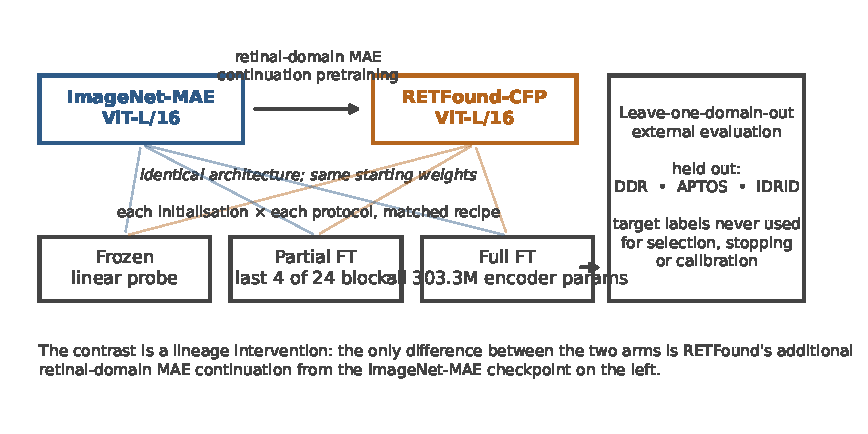
\includegraphics[width=\textwidth]{fig1_study_design.pdf}
%   \caption{[CAPTION --- study design / matched pretraining lineage.
%            Emphasis notes: docs/JBHI_FIGURE_REVIEW.md]}
%   \label{fig:design}
% \end{figure*}
%
% \begin{figure*}[t]\centering
%   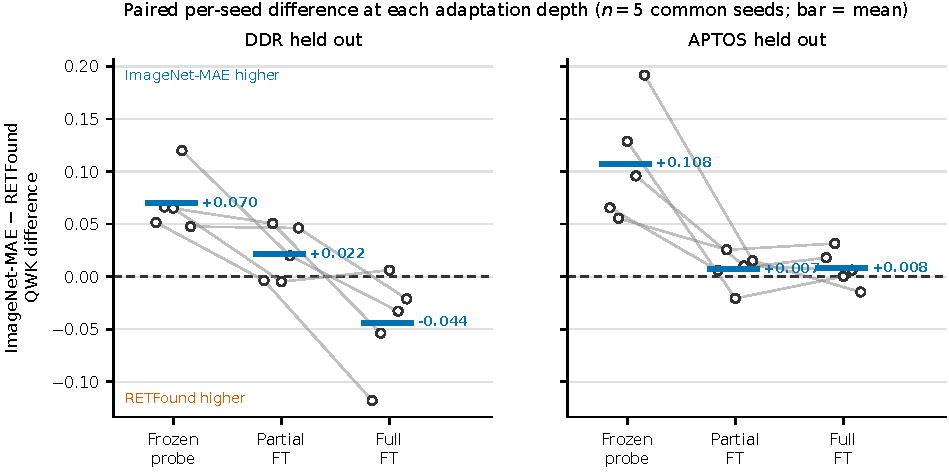
\includegraphics[width=\textwidth]{fig2_adaptation_depth.pdf}
%   \caption{[CAPTION --- adaptation-depth trajectories. Must not imply
%            equivalence near zero.]}
%   \label{fig:depth}
% \end{figure*}
%
% \begin{figure*}[t]\centering
%   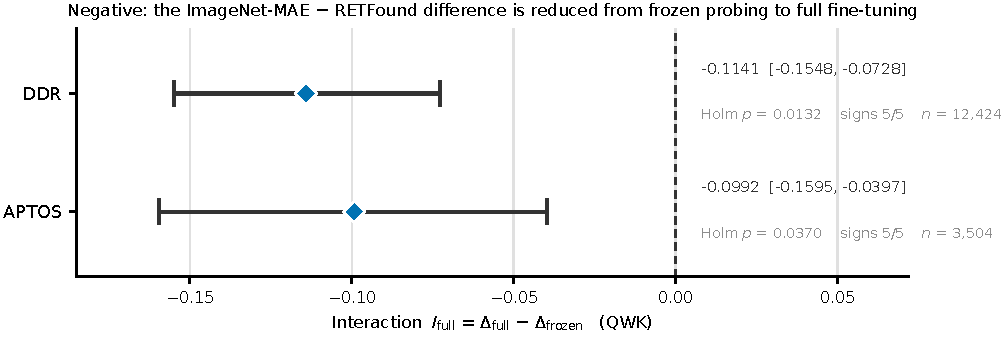
\includegraphics[width=\textwidth]{fig3_primary_interaction.pdf}
%   \caption{[CAPTION --- primary interaction forest. Must state that
%            negative means the difference is REDUCED, not that RETFound
%            won.]}
%   \label{fig:interaction}
% \end{figure*}
%
% \begin{figure*}[t]\centering
%   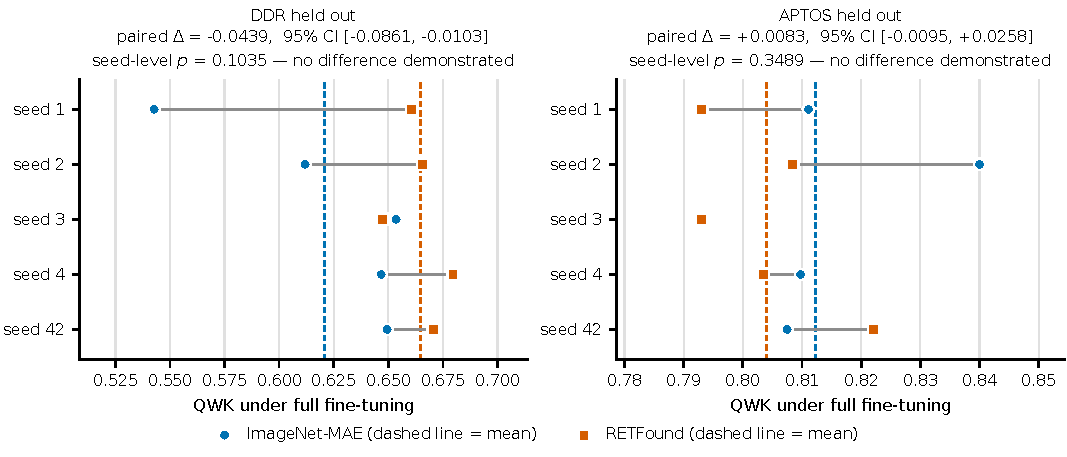
\includegraphics[width=\textwidth]{fig5_full_ft_paired_qwk.pdf}
%   \caption{[CAPTION --- full-FT paired QWK. Must carry the
%            no-difference-demonstrated / not-equivalence wording.]}
%   \label{fig:fullft}
% \end{figure*}
%
% Supplementary: fig4_seed_interaction_slopes.pdf and s1--s6.
% fig4 is the first main-paper candidate to move to the supplement.

% =====================================================================
% TABLES -- reserved placement.
%
% TABLE I   dataset and provenance characteristics
%           source: docs/JBHI_DATASET_PROVENANCE.md
%
% TABLE II  adaptation-depth / matched-model results
%           source: outputs/tables/JBHI_MASTER_RESULTS.tex
%
% TABLE III primary DDR + APTOS protocol interaction
%           source: outputs/tables/JBHI_PRIMARY_INTERACTION.tex
%
% MERGE RECOMMENDATION: keep II and III SEPARATE. See
% docs/JBHI_PAGE_BUDGET.md for the reasoning -- they use different seed
% sets and different inferential status, and merging them invites exactly
% the ten-seed/five-seed confusion the seed_set column exists to prevent.
% =====================================================================

% \begin{table*}[t]
\centering
\caption{Authoritative per-protocol results on the three held-out domains, quadratic weighted kappa. $\Delta$ is the paired ImageNet-MAE minus RETFound difference; intervals are crossed seed $\times$ case bootstrap uncertainty intervals and $p$ is an uncorrected paired seed-level $t$-test. The frozen linear probe was run at ten seeds and the two adaptation protocols at five, so each frozen row appears twice: once over all ten seeds as a descriptive estimate and once over the five seeds common to every protocol. Only the common-five rows may be differenced across protocols, since the interaction is a paired quantity. IDRiD has no full fine-tuning row: that experiment was not run, and no value is imputed for it. Formal multiplicity-adjusted inference in this study attaches to the protocol interaction in Table\~\ref{tab:jbhi-primary-interaction}, not to the per-protocol comparisons here.}
\label{tab:jbhi-master-results}
\begin{tabular}{lllrrrrrrr}
\toprule
Held-out & Protocol & Seed set & $n$ & ImageNet-MAE & RETFound & $\Delta$ & 95\% CI & $p$ & sign \\
\midrule
DDR & Frozen linear probe & all-10 & 10 & 0.5756 & 0.5130 & $+0.0626$ & $[+0.0440, +0.0824]$ & 0.0000 & 10/10 \\
DDR & Frozen linear probe & common-5 & 5 & 0.5805 & 0.5103 & $+0.0702$ & $[+0.0468, +0.0978]$ & 0.0057 & 5/5 \\
DDR & Partial FT (last 4/24) & common-5 & 5 & 0.7183 & 0.6966 & $+0.0217$ & $[-0.0004, +0.0438]$ & 0.1401 & 3/5 \\
DDR & Full fine-tuning & common-5 & 5 & 0.6209 & 0.6648 & $-0.0439$ & $[-0.0861, -0.0103]$ & 0.1035 & 4/5 \\
APTOS & Frozen linear probe & all-10 & 10 & 0.5963 & 0.4829 & $+0.1134$ & $[+0.0787, +0.1493]$ & 0.0001 & 10/10 \\
APTOS & Frozen linear probe & common-5 & 5 & 0.5872 & 0.4796 & $+0.1075$ & $[+0.0623, +0.1536]$ & 0.0121 & 5/5 \\
APTOS & Partial FT (last 4/24) & common-5 & 5 & 0.8334 & 0.8261 & $+0.0073$ & $[-0.0107, +0.0234]$ & 0.4007 & 4/5 \\
APTOS & Full fine-tuning & common-5 & 5 & 0.8123 & 0.8040 & $+0.0083$ & $[-0.0095, +0.0258]$ & 0.3489 & 4/5 \\
IDRiD & Frozen linear probe & all-10 & 10 & 0.6363 & 0.6792 & $-0.0429$ & $[-0.0888, +0.0037]$ & 0.0034 & 9/10 \\
IDRiD & Frozen linear probe & common-5 & 5 & 0.6275 & 0.6701 & $-0.0426$ & $[-0.0959, +0.0131]$ & 0.0497 & 5/5 \\
IDRiD & Partial FT (last 4/24) & common-5 & 5 & 0.7254 & 0.7676 & $-0.0421$ & $[-0.0879, +0.0044]$ & 0.0653 & 5/5 \\
\bottomrule
\end{tabular}
\end{table*}

% \begin{table*}[t]
\centering
\caption{Primary analysis: the protocol-by-initialisation interaction $I_{\text{full}} = \Delta_{\text{full}} - \Delta_{\text{frozen}}$ on the two held-out domains for which matched full fine-tuning was run, over the five common seeds. $\Delta$ is ImageNet-MAE minus RETFound QWK within a protocol, so a negative interaction means the ImageNet-MAE advantage measured under frozen probing is reduced once the encoder adapts. Intervals are crossed seed $\times$ case bootstrap uncertainty intervals and are not tests; $p$ is the paired seed-level $t$-test, Holm-adjusted across exactly these two domains; $p_{\text{flip}}$ is an exact sign-flip sensitivity analysis whose smallest attainable two-sided value at five seeds is $0.0625$. Both domains are statistically supported under the study's inferential framework, with all five seed-level interactions negative on each. No pooled two-domain $p$-value is reported: the test sets differ in size and shift structure. The APTOS analysis was specified as a confirmatory replication after the DDR result was frozen, and Holm adjustment across the two is applied for final reporting.}
\label{tab:jbhi-primary-interaction}
\begin{tabular}{lrrrrrrrrr}
\toprule
Held-out & $n_{\text{test}}$ & seeds & $\Delta_{\text{frozen}}$ & $\Delta_{\text{full}}$ & $I_{\text{full}}$ & 95\% CI & $p$ & $p_{\text{Holm}}$ & $p_{\text{flip}}$ & sign \\
\midrule
DDR & 12\,424 & 5 & $+0.0702$ & $-0.0439$ & $-0.1141$ & $[-0.1548, -0.0728]$ & 0.0066 & 0.0132 & 0.0625 & 5/5 \\
APTOS & 3\,504 & 5 & $+0.1075$ & $+0.0083$ & $-0.0992$ & $[-0.1595, -0.0397]$ & 0.0370 & 0.0370 & 0.0625 & 5/5 \\
\bottomrule
\end{tabular}
\end{table*}


\bibliographystyle{IEEEtran}
\bibliography{refs_jbhi_verified}

\end{document}
